\graphicspath{ {./images} }

%!TEX root = ../thesis.tex
\chapter{Methods}
\label{ch:methods}

\section{The Simulink Model}
\begin{figure}
	\centerline{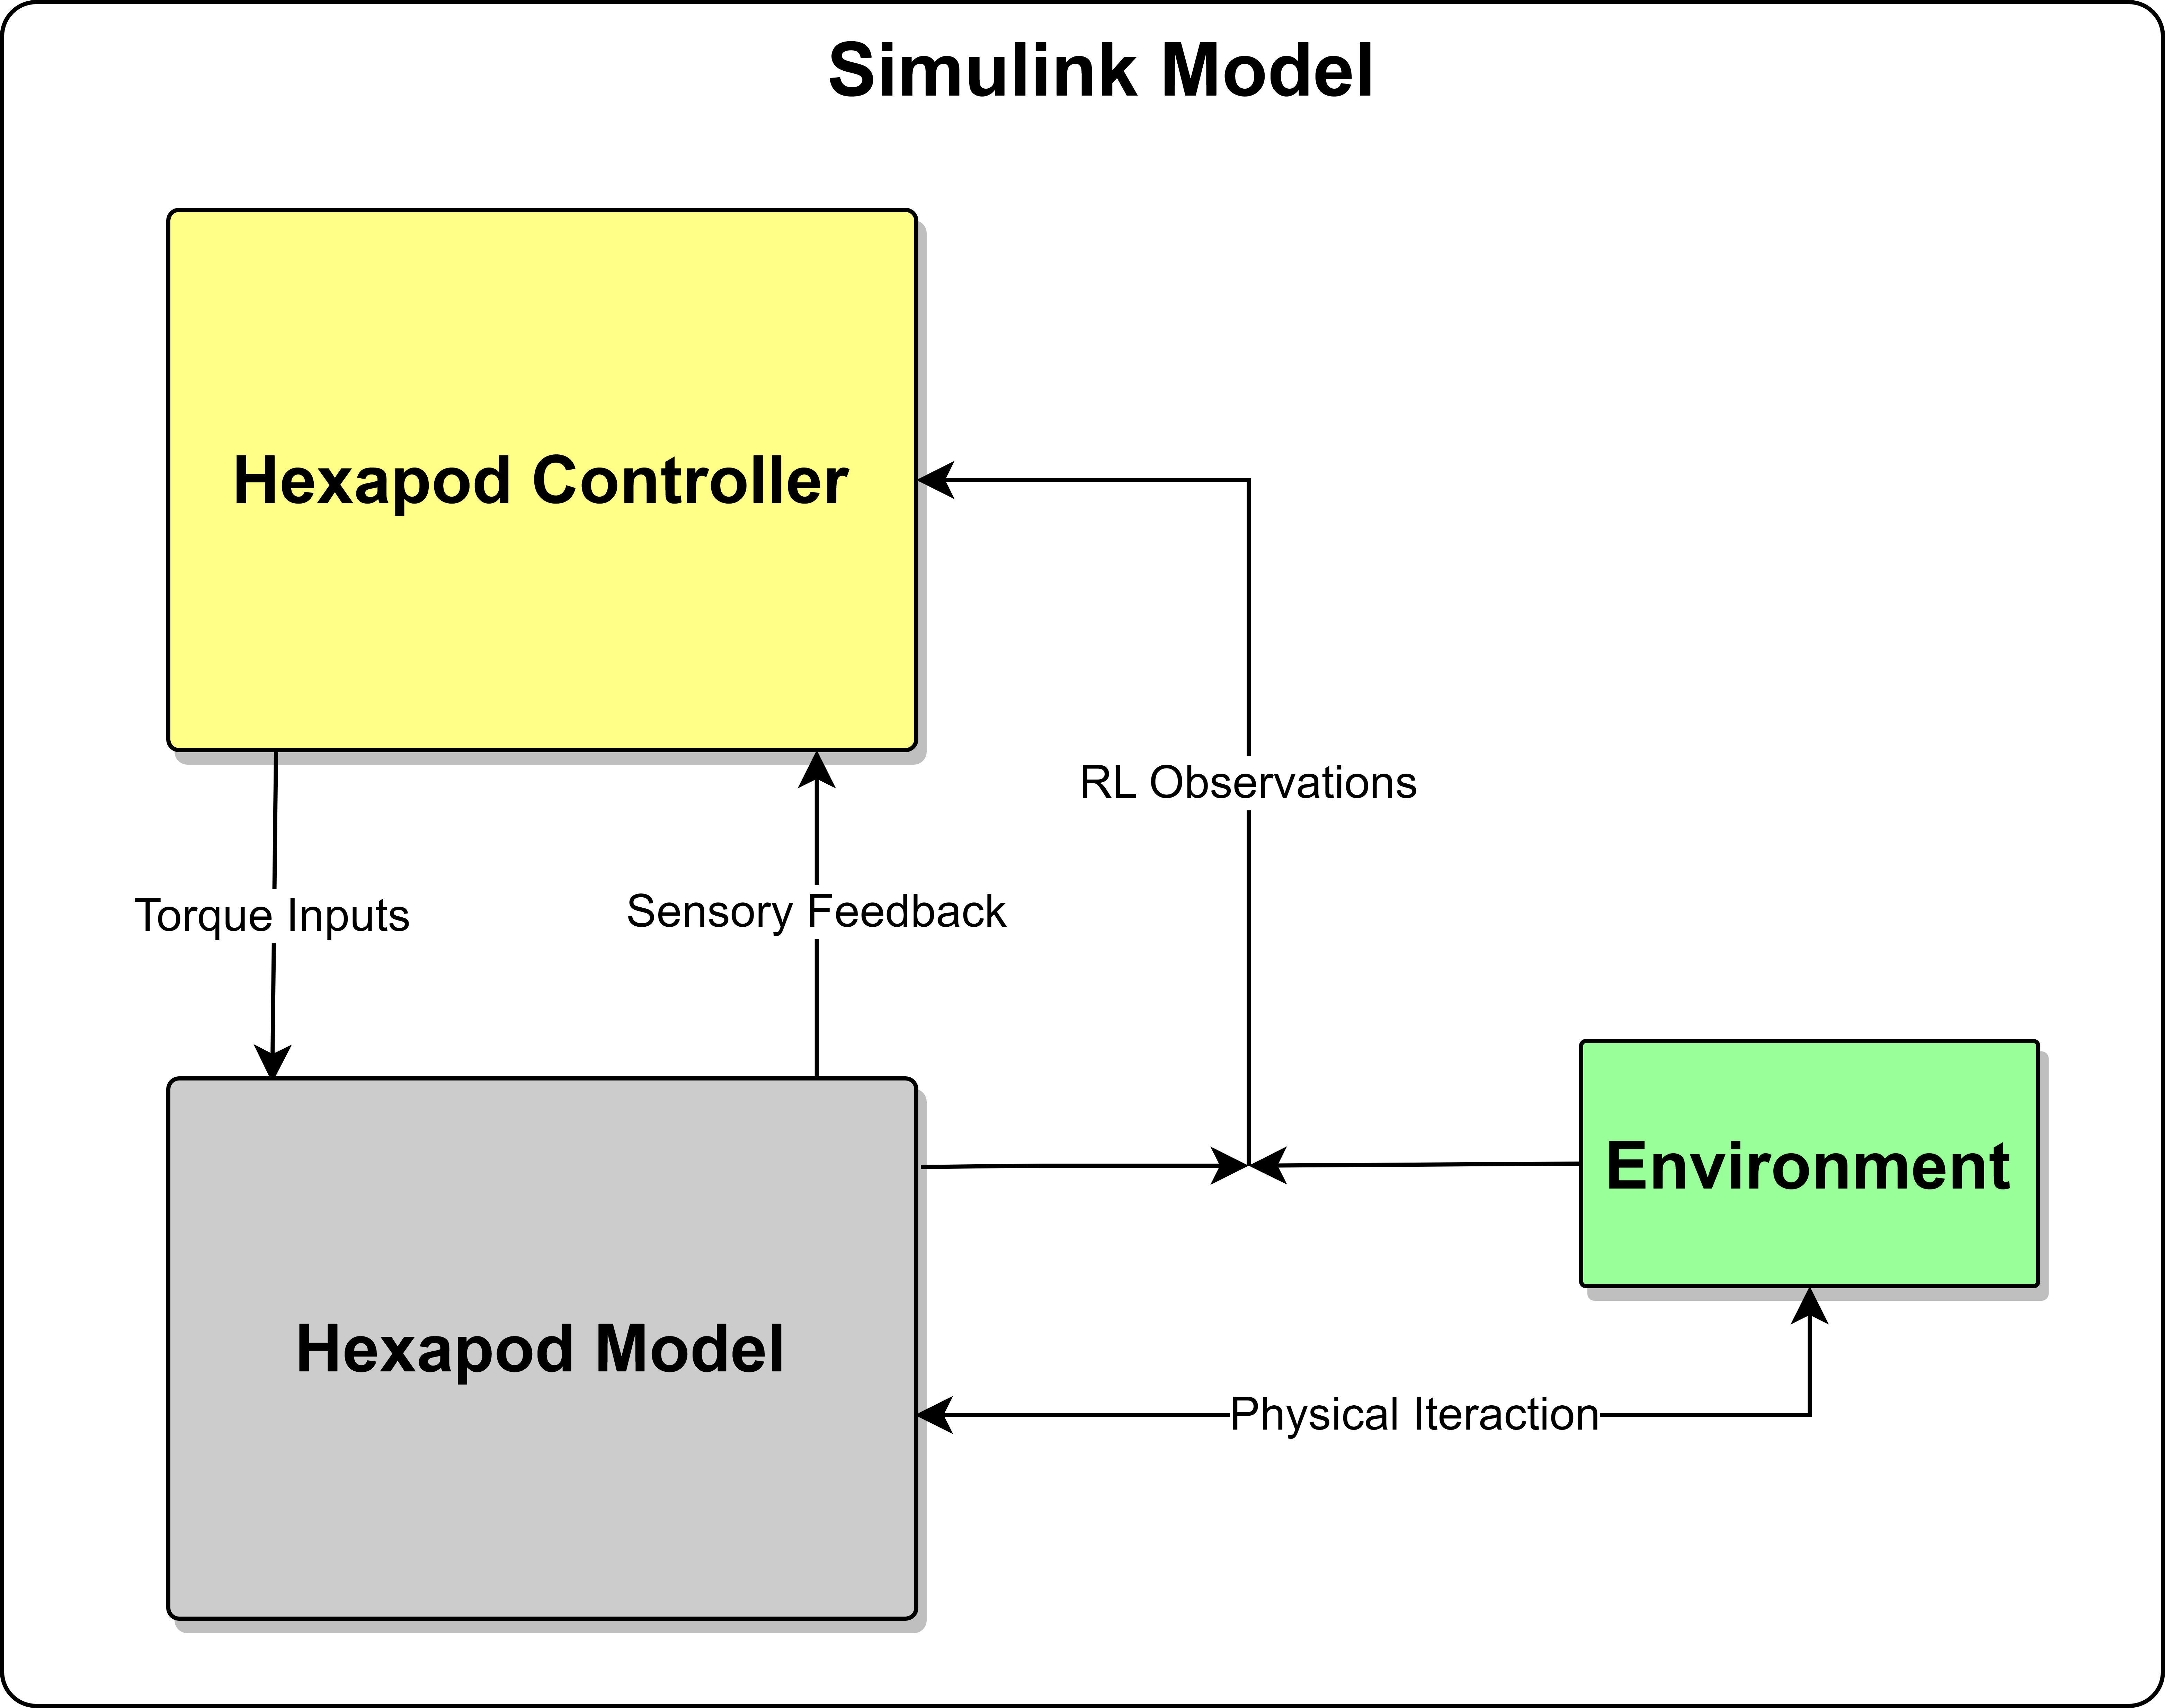
\includegraphics[scale=0.035]{HexapodModel_Overview}}
	\caption{Simulink Model Overview}
	\label{figure: Simulink Model Overview}
\end{figure}

\subsection{Model of the Hexapod}

\begin{figure}
	\centerline{\includesvg[scale=0.7]{Simulink/Simulink_PhysicalHexapodOverview}}
	\caption{Hexapod Model Overview}
	\label{figure: Hexapod Model Overview}
\end{figure}

\begin{figure}
	\centerline{\includesvg[scale=0.6]{Simulink/Simulink_HexapodLegOverview}}
	\caption{Model of Hexapod Leg}
	\label{figure: Hexapod Leg}
\end{figure}


The hexapod model we used in this work is the \textit{PhantomX MK4} developed by \textit{Trossen Robotics}.
The company provides a .urdf file(Unified Robotics Description Format) of the robot which is imported into the MATLAB environment.
MATLAB is then able to convert the file into a Simulink model consisting of blocks from the Simscape library.

\todo{Insert images of hexapod model}
The main body of the hexapod robot is represented by a rigid body and a main coordinate frame.
Each of the robots legs consists of 3 rigid bodies(coxa, femur and tibia) which are connected to each other by 2 joints.
A third joint then attaches the coxa, and thus the whole leg, to the main body.
Each joint has 1 (rotational) DoF.
To position each rigid body and joint correctly, so called rigid transformations are used to translate and rotate each part.

Each of the models joints can receive a torque to be applied as input and output various sensory data such as the joints position, velocity and acceleration. 
To simplify the model, we did not model the physical servo motors and instead used this direct torque input to the joints.

From a top level perspective, the hexapod model consists of the main body(thorax) and the 6 legs.
This system receives as input the torque to be applied on each joint and outputs sensory data taken from these joints, namely the joints position, velocity and acceleration.
In this work only the data about the current joint positions is utilized, but to allow for further expansion on the model, such as optimizing for minimal energy consumption, joint velocity and acceleration are provided as well.
Integration of the joint position over time would yield the same result, but we decided for ease of use to include the data explicitly.

To encapsulate the system and only provide the necessary inputs and outputs, the system is placed inside a subsystem.
This also allows for the duplication of the hexapod system, so that in future research it can also be used in multi-agent simulations.

\subsection{Environment}
To validate the robot model and to provide a place for the robot to learn the coordination rules of its legs, we constructed a simple test environment.
The environment currently only consists of a horizontal plane, but can expanded to include more complex terrain with little effort.
Some examples which we experimented with but did not include in this thesis are inclined planes and also obstacles on the ground.

\subsection{Controller}
The controller is responsible for the hexapods locomotion.
It controls the movement of the robots six legs according to a predefined gait.
As inputs, the controller receives the sensory data from the hexapod model.
According to this data the controller outputs the torques to be applied to each joint.

\begin{figure}
	\centerline{\includegraphics[scale=0.03]{HexapodController}}
	\caption{Controller Overview}
	\label{figure: Controller Overview}
\end{figure}
Each of the hexapods legs is controlled by a separate control unit which receives the information of the legs joint sensors as input and computes the torques to be applied to its joints as output.
The control unit for a leg receives the frequency for the swing-stance cycle, duty-percentage of the swing phase and swing-initiation signal as coordination inputs.
This information can either come from a static gait definition, in which the parameters for each leg are statically configured, or can be provided by a reinforcement learning agent.
The agent receives observations from the environment and hexapod model as well as a reward signal and outputs actions in the form as mentioned above.

\begin{figure}
	\centerline{\includesvg[scale=0.6]{Simulink/Simulink_LegControllerOverview}}
	\caption{Control unit for a single leg}
	\label{figure: Leg control unit}
\end{figure}

A single leg control unit, as seen in \ref{figure: Leg control unit}, consists of a leg trajectory generator and one PID feedback control loop for each of the 3 leg joints.
The leg trajectory generator is responsible for generating a path for the leg to follow according to the input frequency, duty cycle swing initiation and pattern rotation.
It outputs the desired angle for the \textalpha-, \textbeta- and \textgamma-joints, which the PID controllers are then trying to achieve.
The PID controller parameters $K_p$, $K_i$ and $K_d$ (and $N$) are tuned via trial-and-error method and are depicted in \ref{table: PID parameters}.

\begin{figure}
	\centerline{\includesvg[scale=0.75]{Simulink/Simulink_LegTrajectoryGenerationOverview}}
	\caption{Leg trajectory generator}
	\label{figure: Leg trajectory generator}
\end{figure}

The leg trajectory generator, as seen in \ref{figure: Leg trajectory generator}, consists of a signal generator, a pattern rotation subsystem and an analytic inverse kinematics solver.
The signal generator is responsible for creating a continuous leg trajectory given as x- and z-coordinates.
The pattern rotation subsystems rotates, if required, the x-z-trajectory around the z-axis to allow for omni-directional movement of the robot.
At the end of the trajectory generation the inverse kinematics block receives the trajectory coordinates and translates them into joint angles.
Even though Simulinks \textit{Robotics System Toolbox} includes an iterative IK-solver, we decided to implement our own analytical solver to increase simulation speed.
Due to the nature of an iterative solver, the calculation time required is significantly higher than that of a purpose-build analytical solver, in our case about x to y times faster.

\begin{figure}
	\centerline{\includesvg[scale=0.85]{Simulink/Simulink_SignalGeneratorOverview}}
	\caption{Signal Generator}
	\label{figure: Signal Generator}
\end{figure}

A Signal Generator, as seen in \ref{figure: Signal Generator}, consists two parts, a swing phase subsystem and a stance phase subsystem.
The stance subsystems provide the x- and z-coordinate signal during stance, the swing subsystem during swing.
The coordination between these two units is influenced by the cycle frequency, duty factor and swing initiation signal.
If the swing initiation is pulled high, the swing phase subsystem is reset(so it starts from the beginning) and the outputs(x,z) are switched to the swing system.
When the swing phase is finished, meaning the x-coordinate coincides with the AEP, the swing phase subsystem gives up control the the stance phase subsystem via the \textit{Swing finished} signal.
This induces a reset on the stance phase subsystem and switches the outputs over to this system.

\begin{table}
	\centering
	\begin{tabular}{| c | c |}
		\hline
		parameter & value\\
		\hline
		$K_p$ & ... \\
		\hline
		$K_i$ & ... \\
		\hline
		$K_d$ & ... \\
		\hline
		$N$ & ... \\
		\hline
	\end{tabular}
	\caption{Gain parameters used for pid-tuning}
	\label{table: PID parameters}
\end{table}

\begin{table}
	\centering
	\begin{tabular}{| c | c | c | c |} 
		\hline
		 & \textbf{\textalpha} & \textbf{\textbeta} & \textbf{\textgamma} \\ [0.5ex] 
		\hline
		left front, right back & 45 & 14.03624347 & 60.58440117  \\ 
		\hline
		left/right middle & 0 & 14.03624347 & 60.58440117 \\
		\hline
		right front, left back & -45 & 14.03624347 & 60.58440117 \\
		\hline
	\end{tabular}
	\caption{Initial joint positions according to urdf-file}
	\label{table:Initial joint positions}
\end{table}




\todo{Viel tiefer ins Detail gehen}
\todo{Bilder}

\section{Learning Leg Coordination}
The leg coordination problem can be considered a Markov decision process(MDP).
The MDP is a 5-tuple $\mathcal{\{S,A,P,R,\gamma\}}$, where $\mathcal{S}$ is a finite set of states, $\mathcal{A}$ is a finite set of actions, $\mathcal{P}$ is a state-transition probability matrix ($\mathcal{P}_{ss'}^a=\mathbb{P}[S_{t+1}=s' | S_t=s, A_t=a]$), $\mathcal{R}_s^a$ is a reward function ($\mathcal{R}_s^a = \mathbb{E}[R_{t+1} | S_t=s, A_t=a]$) and $\gamma \in [0,1]$ is a discount factor.


